\chapter{Experimentos}

En capítulos anteriores se han expuesto los objetivos marcados para la realización del proyecto así como la solución desarrollada para cada uno de estos problemas y las herramientas utilizadas para los mismos. En este capítulo se muestran los experimentos que se han ido realizando según íbamos cumpliendo objetivos y que sirven como validación experimental de la solución programada.\\

\section{Experimentos con simulador Gazebo}

Una vez desarrollado el proyecto y satisfaciendo todos los objetivos marcados se han realizado pruebas sobre el drone simulado en Gazebo para comprobar sin ningún tipo de riesgos el funcionamiento del mismo.\\

\begin{figure}[h!]
\centering
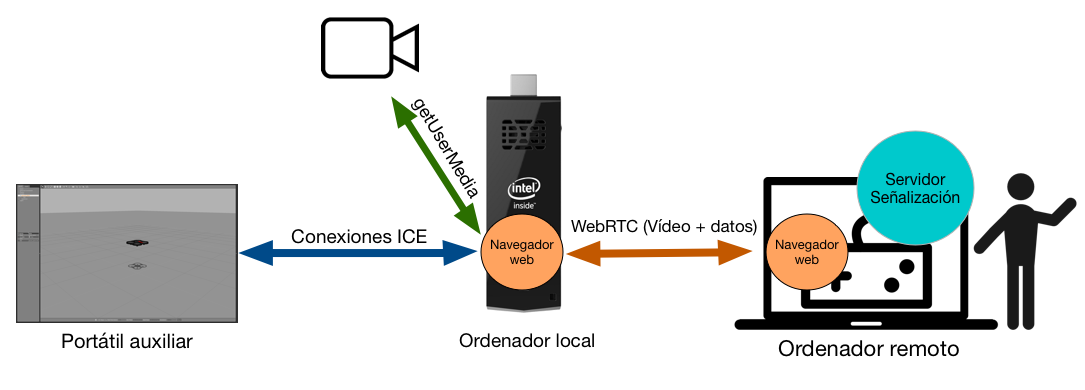
\includegraphics[width=0.9\textwidth]{experimento1}
\caption{Experimento con el simulador Gazebo y un ordenador remoto.}
\label{fig:esquemaexperimento1}
\end{figure}

Para realizar este experimento de la manera más realista al experimento final con el drone real se ha utilizado un \emph{Intel Compute Stick}\footnote{\url{http://www.intel.com/content/www/us/en/compute-stick/compute-stick-product-brief.html}} como par local. El navegador en ese \emph{computer stick} es el encargado de conectarse a las interfaces ICE que nos proporciona el plugin ArDrone desarrollado por JdeRobot para el simulador Gazebo. Este ordenador está compuesto por un procesador Intel Atom que corre Ubuntu 14.04 LTS como sistema operativo. El simulador Gazebo se ha ejecutado en un portátil auxiliar y utilizaremos otro equipo portátil como par remoto desde el que teleoperaremos el drone además de ejecutar el servidor de señalización. La figura \ref{fig:esquemaexperimento1} muestra el esquema del montaje de este experimento. \\

Los resultados de este experimento han sido muy positivos, el control y manejo del drone han sido de manera fluida y sin realizar ningún movimiento extraño producido por algún tipo de mal funcionamiento del código. El manejo se ha realizado tanto con los \emph{joysticks} virtuales como con el mando. Se puede ver un fotograma del vídeo\footnote{\url{http://jderobot.org/Irodmar-tfg#WebRTC_on_a_drone_working_with_Gazebo5}} del experimento en la figura \ref{fig:experimentogazebo}.\\

\begin{figure}[h!]
\centering
\includegraphics[width=0.9\textwidth]{experimentogazebo}
\caption{Experimento con el simulador Gazebo.}
\label{fig:experimentogazebo}
\end{figure}

En la siguiente figura (\ref{fig:secexp1}) se puede observar la secuencia de movimiento del drone durante el experimento.\\

\newpage
\begin{figure}[h!]
\centering
  \begin{subfigure}[]{47mm}
    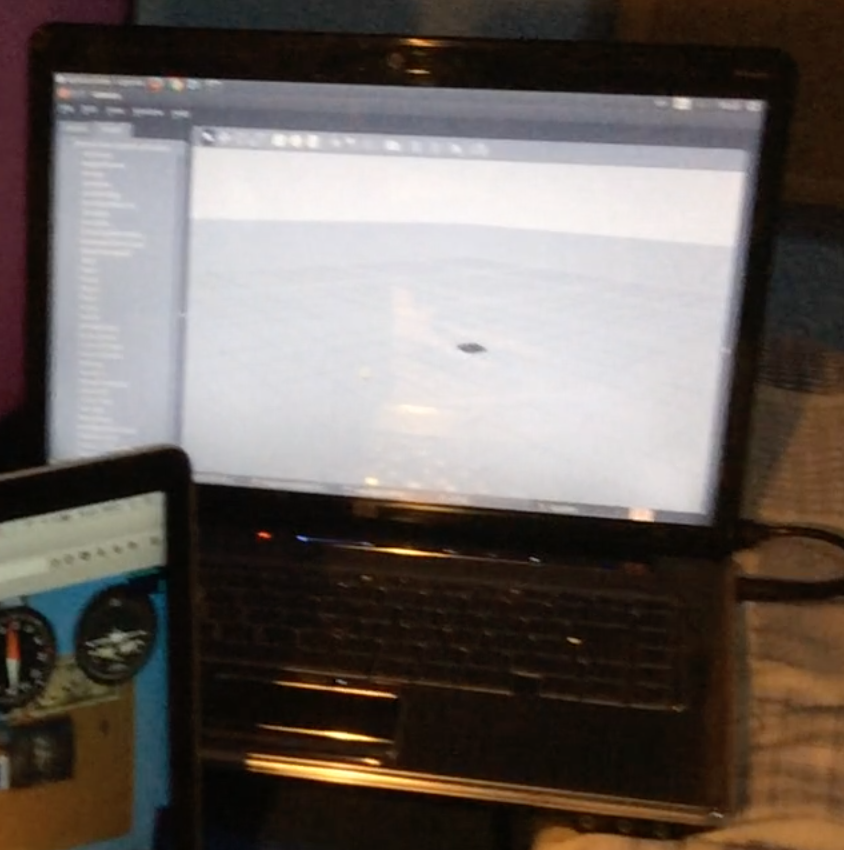
\includegraphics[width=47mm]{sec_exp1_1}
  \end{subfigure}
  \hspace{0.5pt}
  \begin{subfigure}[]{47mm}
    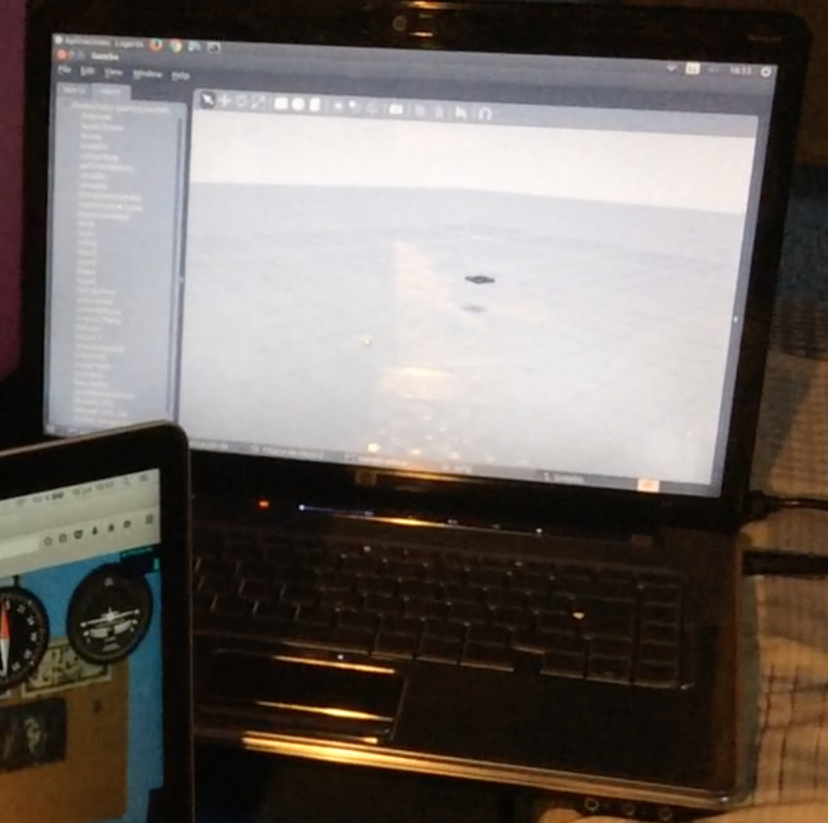
\includegraphics[width=47mm]{sec_exp1_2}
  \end{subfigure}
    \hspace{0.5pt}
    \begin{subfigure}[]{47mm}
    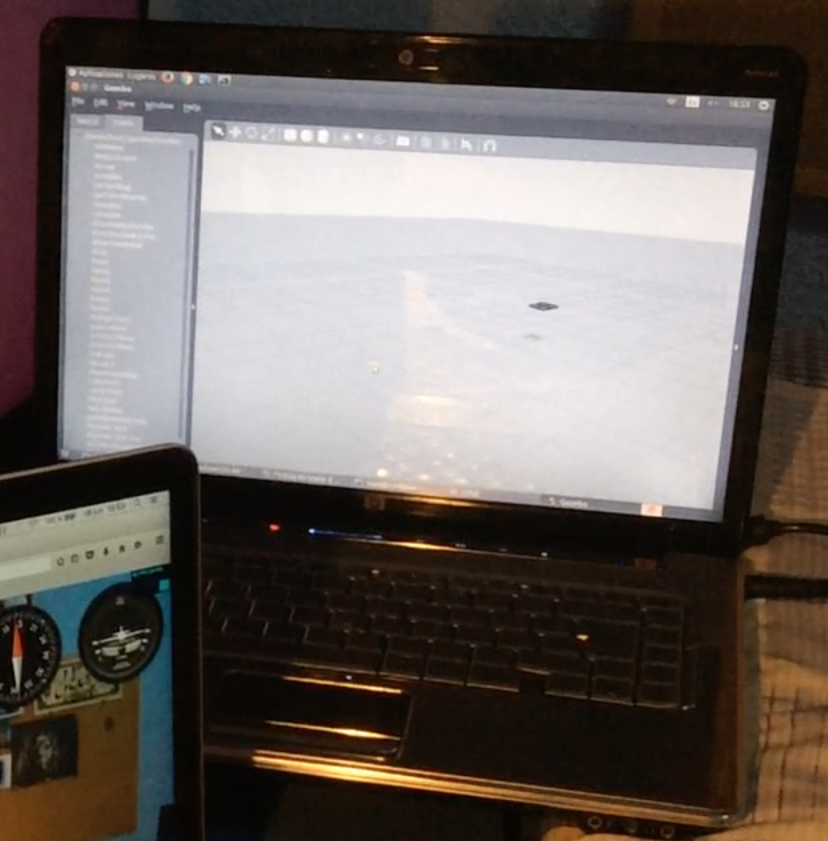
\includegraphics[width=47mm]{sec_exp1_3}
  \end{subfigure}
    \caption{Secuencia de movimiento del drone dentro de Gazebo.}
  \label{fig:secexp1}
\end{figure}


\section{Vuelo del drone real}

Las pruebas con el drone real se han divido a su vez en dos. La primera consiste en realizar las pruebas sin colocar a bordo del drone ni el \emph{computer stick} ni la cámara. Ambos se han usado para las pruebas pero para una primera aproximación se han realizado sin estar a bordo.\\

\begin{figure}[h!]
\centering
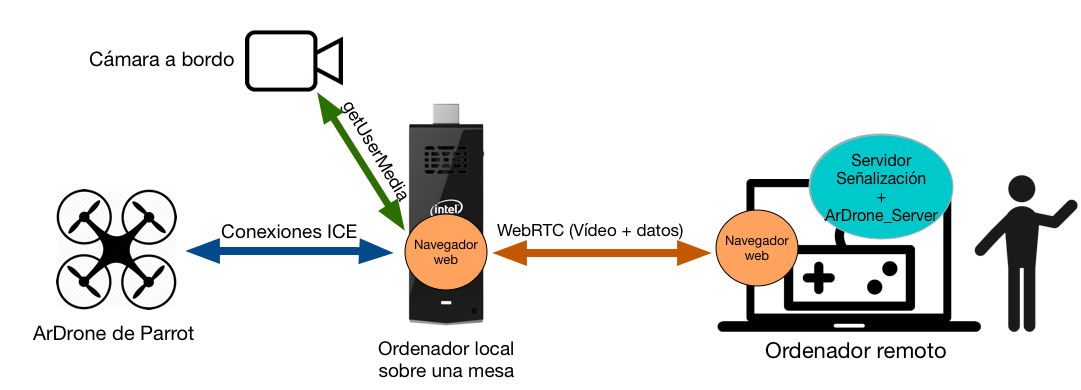
\includegraphics[width=0.9\textwidth]{esquema_experimento2}
\caption{Esquema del experimento con el drone real.}
\label{fig:esquemaexperimento2}
\end{figure}

Así pues la distribución de los equipos es como se muestra en la figura \ref{fig:esquemaexperimento2}: computer stick como par local, que se conecta al drone real y accede a la cámara USB conectada al mismo, y ordenador portátil como par remoto desde el que se teleoperará el drone y a su vez está ejecutando el servidor de señalización y el \texttt{ardrone\_server.}\\

La figura \ref{fig:experimentodronereal1} muestra la realización de este experimento. En la mediawiki\footnote{\url{http://jderobot.org/Irodmar-tfg\#First\_Flying\_with\_Real\_Drone}}\cite{Mediawiki} hay un vídeo completo del mismo. En la figura \ref{fig:secexp2} se ha representado con tres imágenes la secuencia de vuelo del drone durante el experimento.\\

\begin{figure}[h!]
\centering
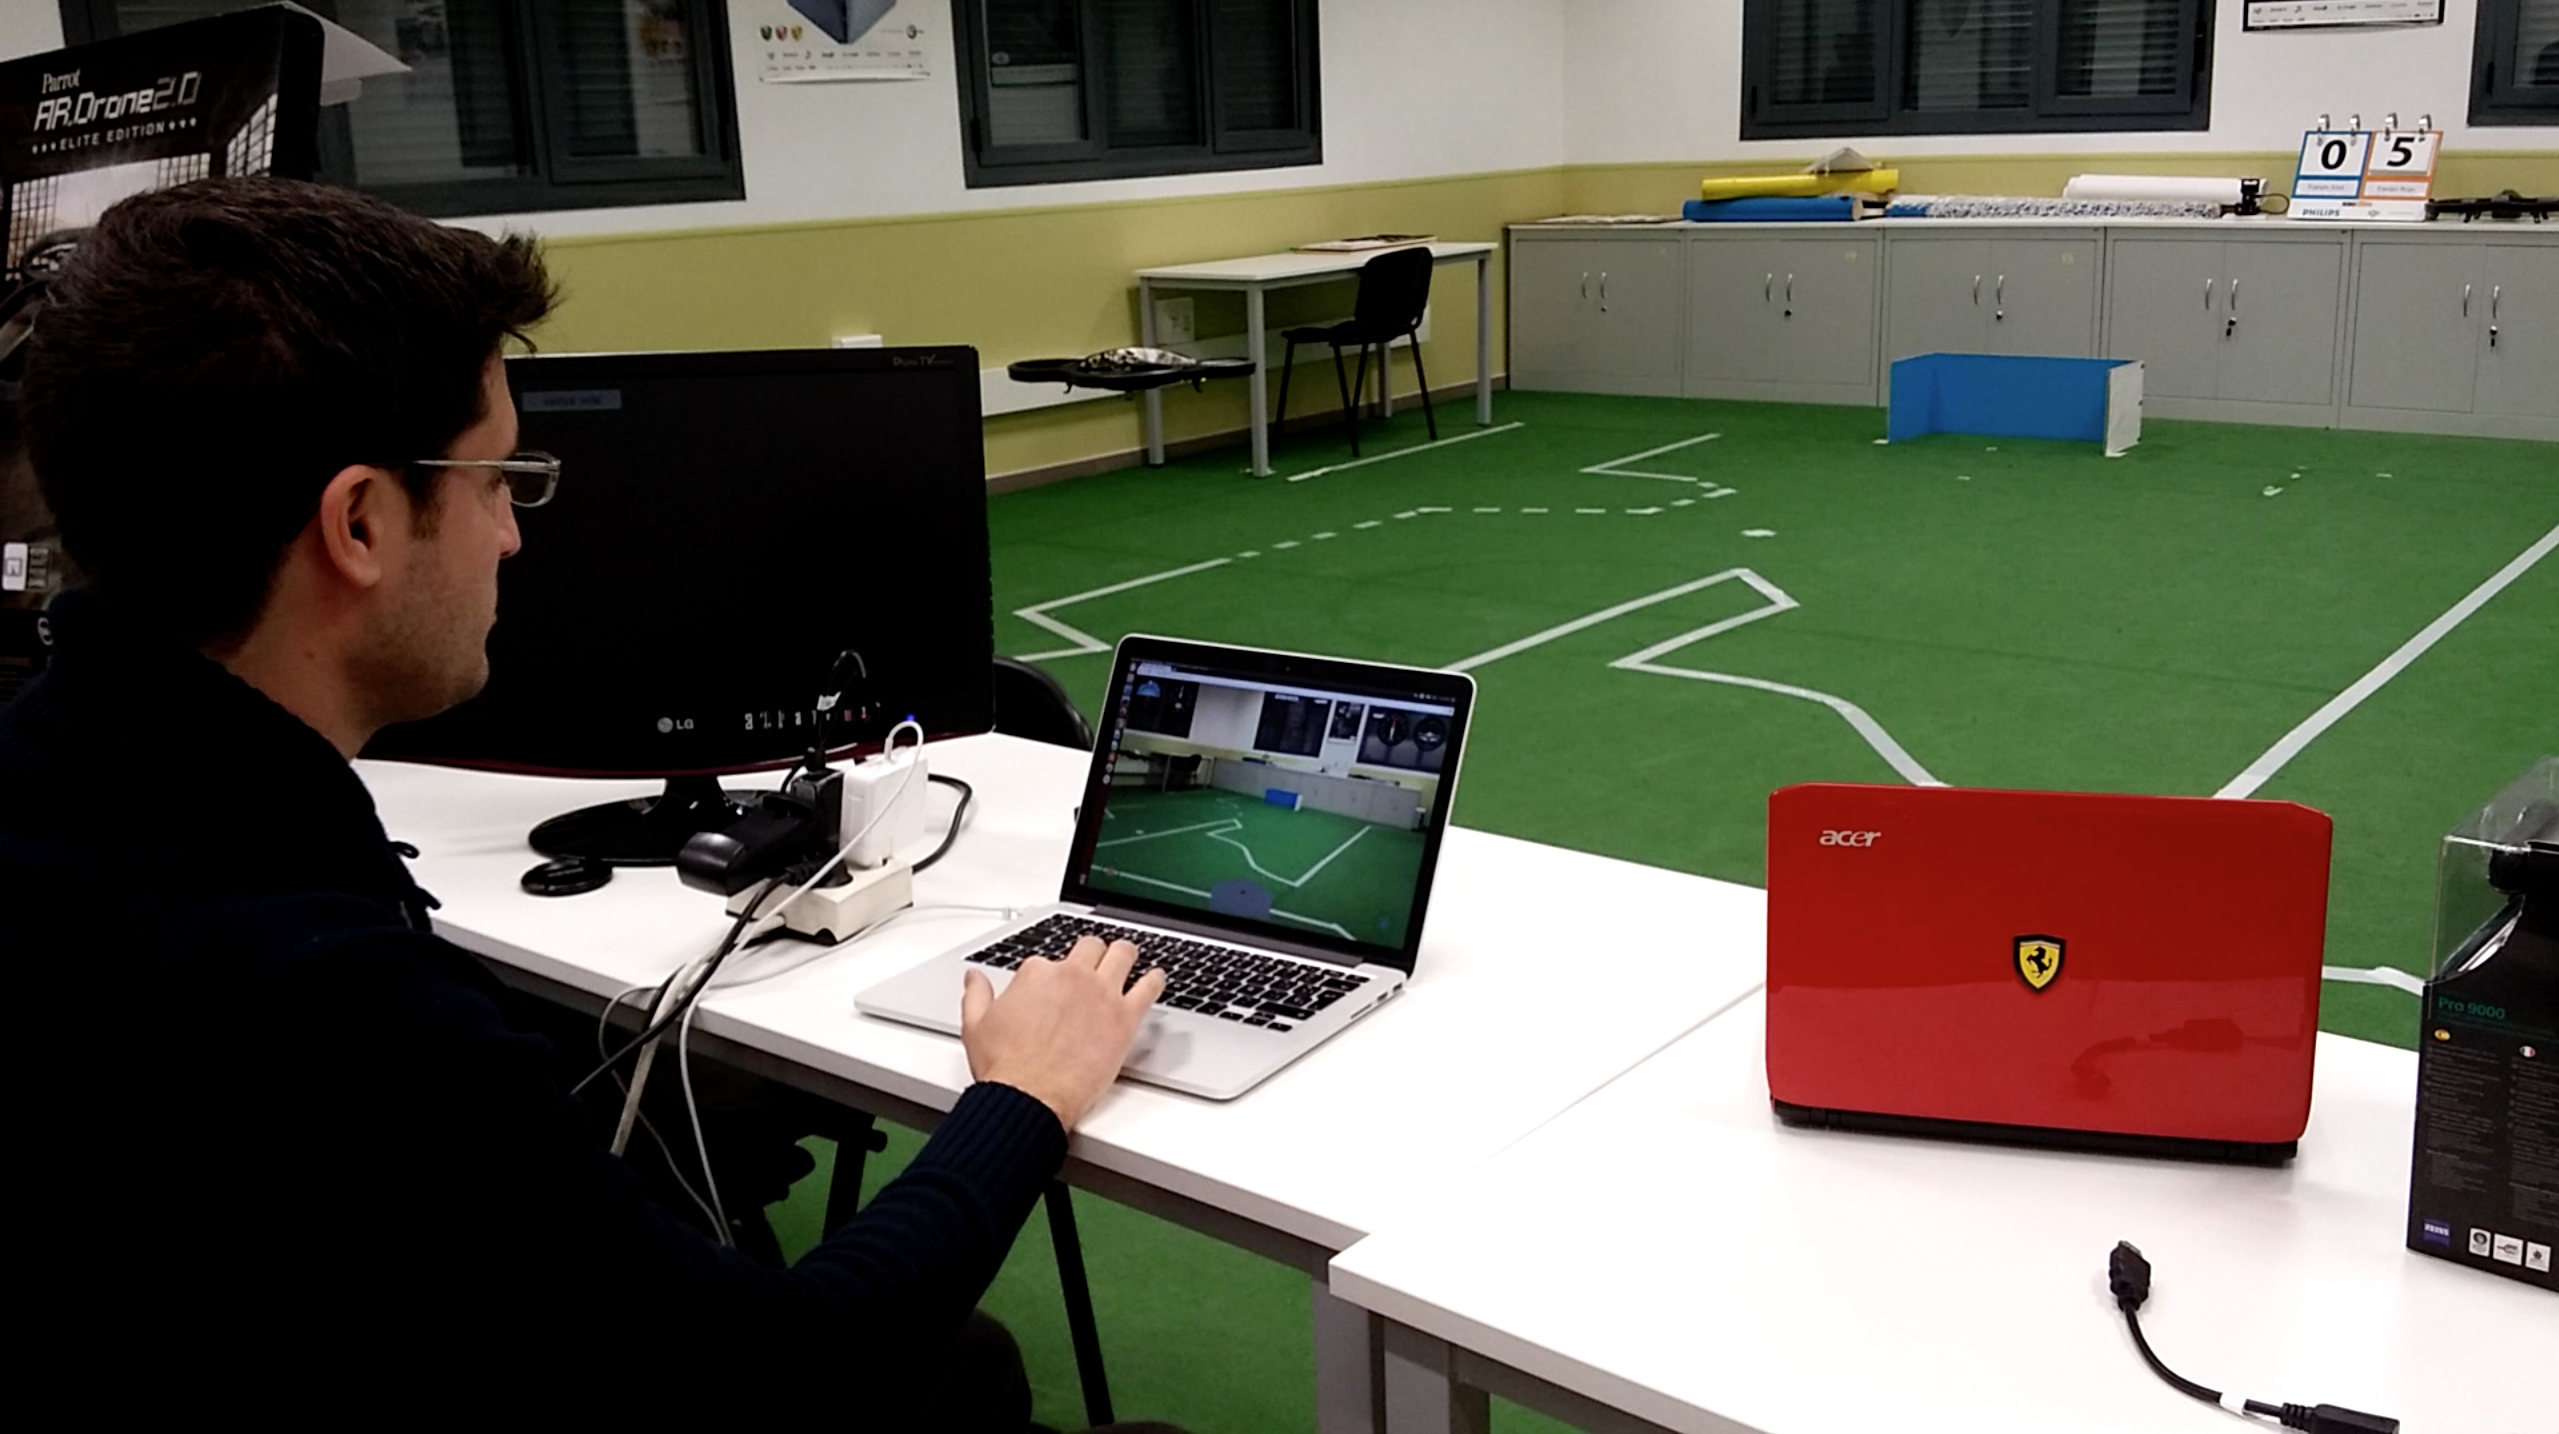
\includegraphics[width=0.9\textwidth]{experimentodronereal1}
\caption{Experimento uno con drone real.}
\label{fig:experimentodronereal1}
\end{figure}


\begin{figure}[h!]
\centering
  \begin{subfigure}[]{48mm}
    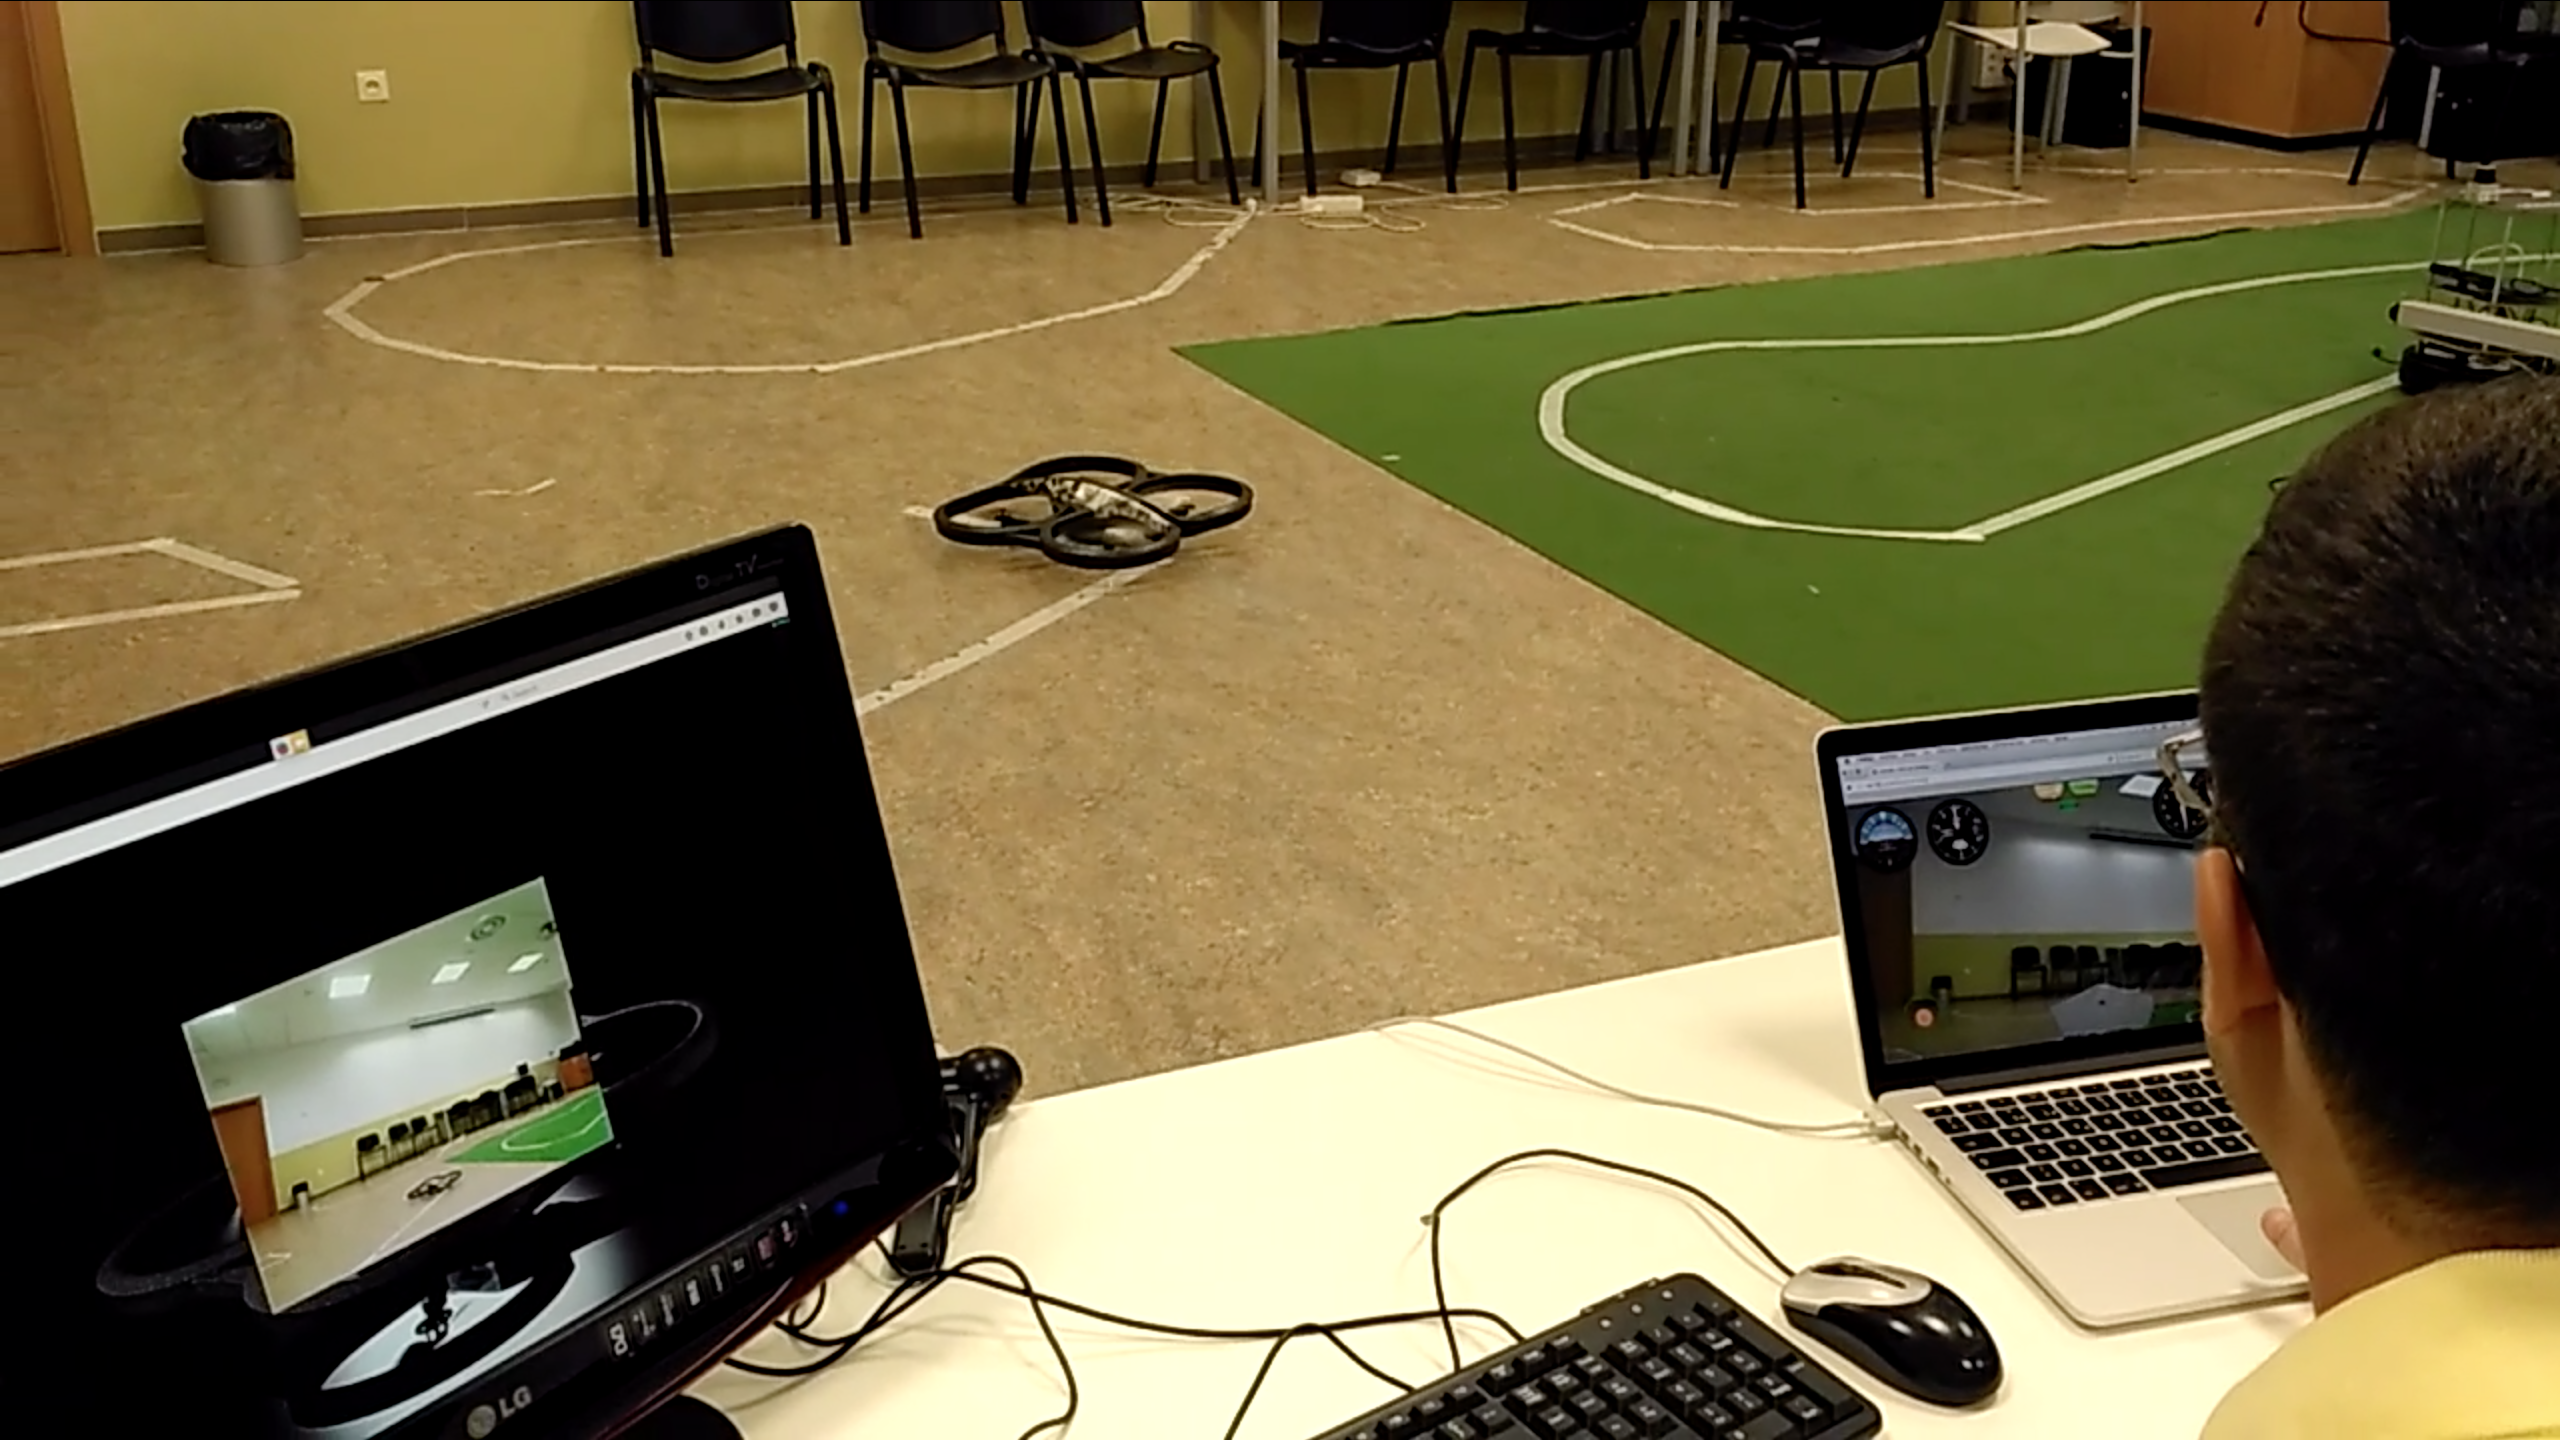
\includegraphics[width=48mm]{sec_exp2_1}
  \end{subfigure}
  \hspace{1pt}
  \begin{subfigure}[]{48mm}
    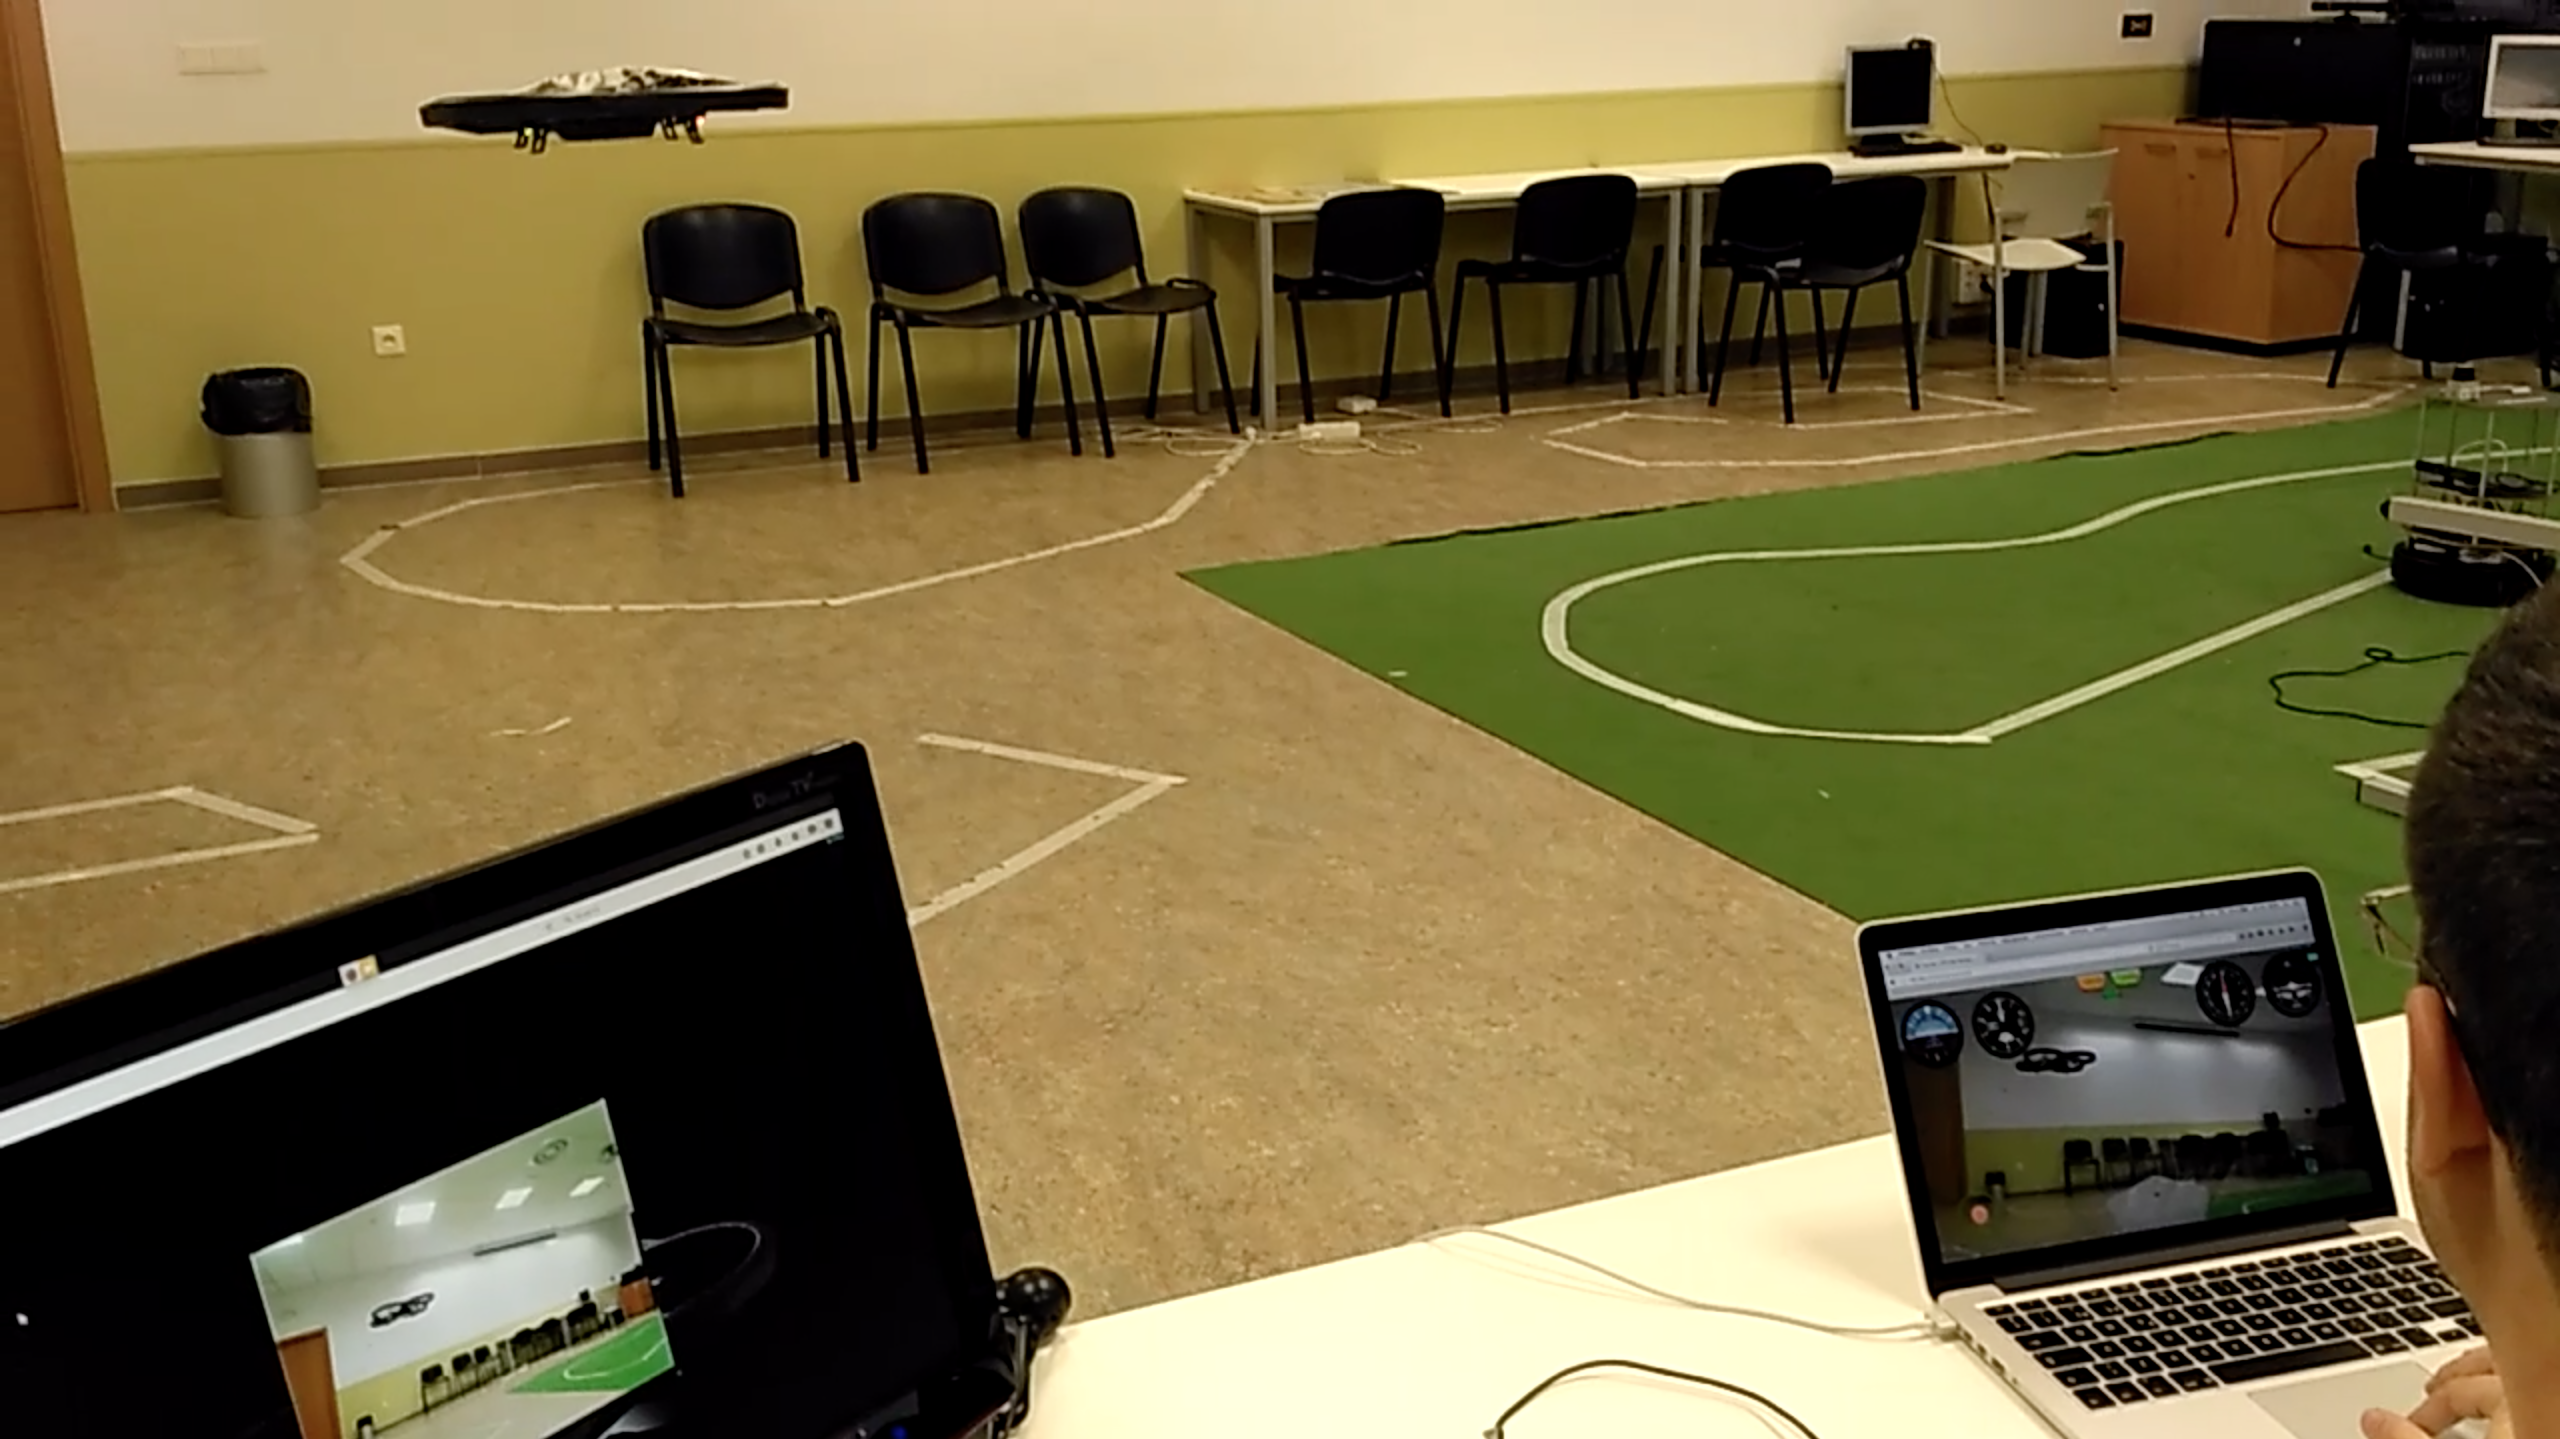
\includegraphics[width=48mm]{sec_exp2_2}
  \end{subfigure}
    \hspace{1pt}
    \begin{subfigure}[]{48mm}
    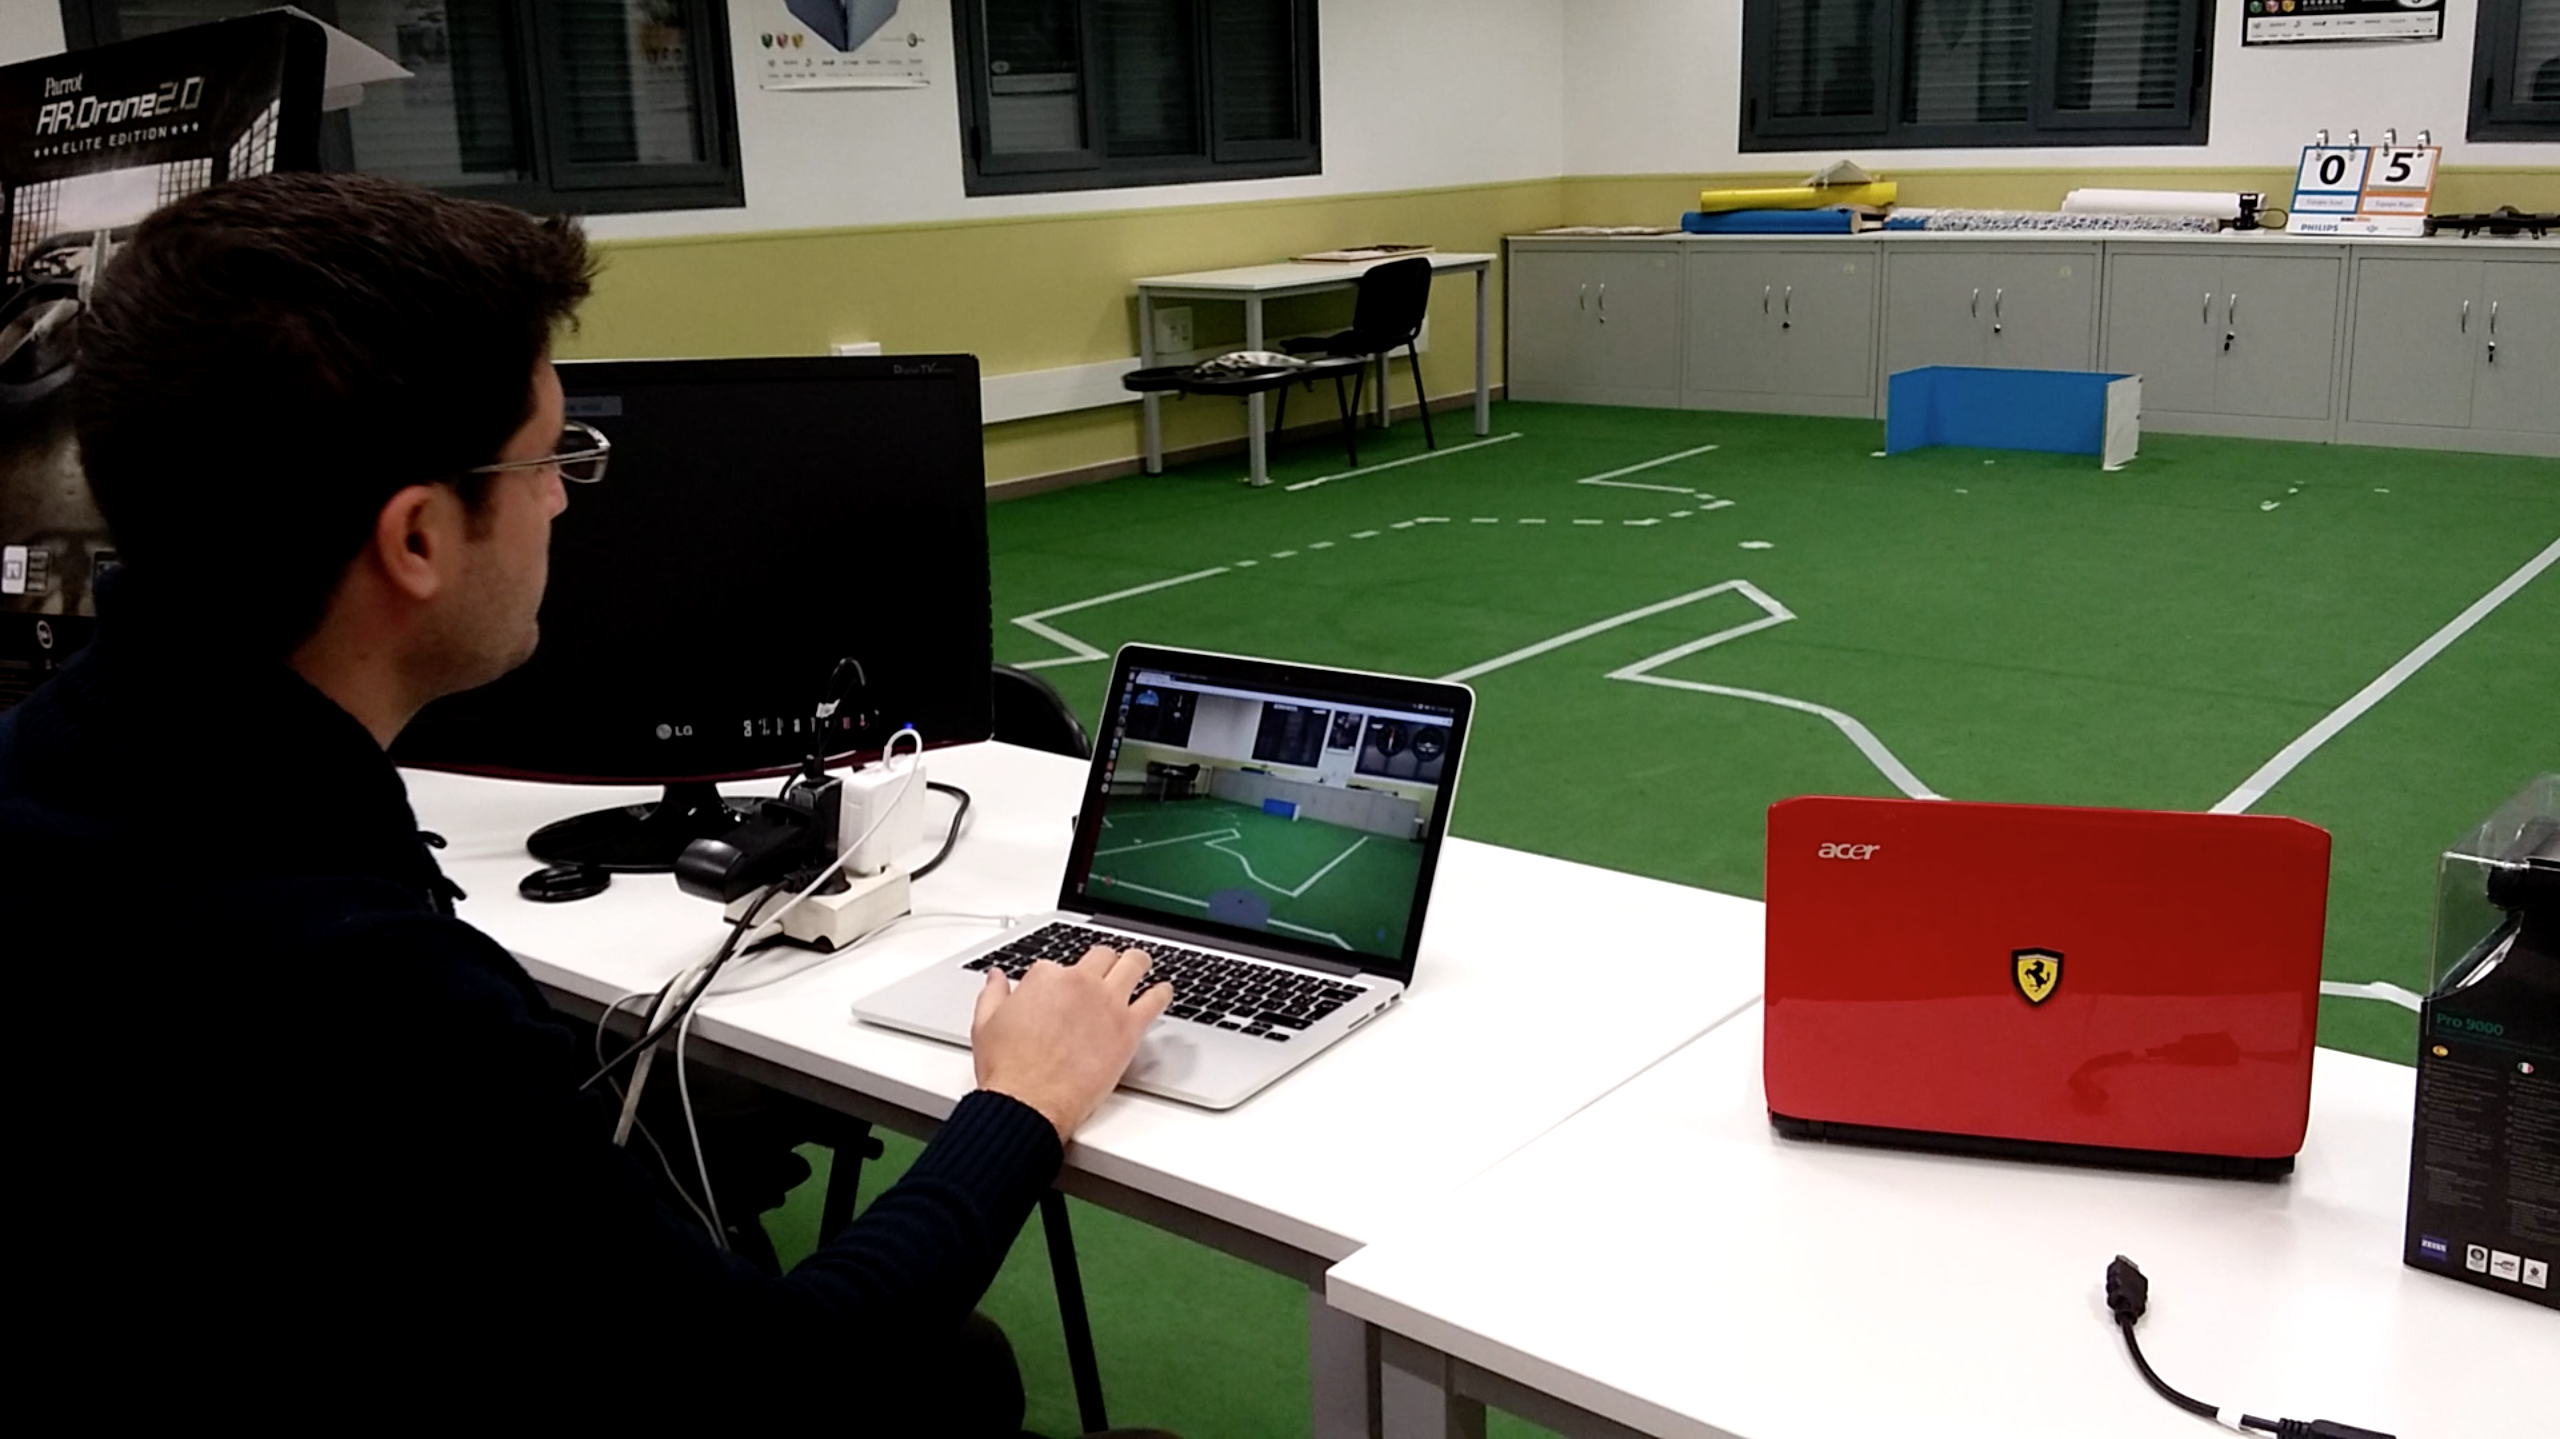
\includegraphics[width=48mm]{sec_exp2_3}
  \end{subfigure}
    \caption{Secuencia de movimiento del experimento con el drone real.}
  \label{fig:secexp2}
\end{figure}


Esta prueba también ha sido un éxito, por lo que nos marcamos el siguiente experimento con el \emph{computer stick} y la cámara a bordo del drone. Este experimento la configuración es la misma que en el anterior, pero el manejo del drone con la aplicación será más realista ya que tenemos la cámara en primera persona.\\


La segunda prueba realizada ha consistido en colocar a bordo del drone la cámara, el \emph{computer stick}, el cuál actuará como par local, estableciendo la conexión con el drone y accediendo a la cámara. El drone tiene una conexion USB de salida pero la potencia no es suficiente para hacer funcionar el \emph{computer stick}. Por este motivo se ha tenido que colocar a bordo una pila adicional la cual hará las veces de fuente de alimentación. Por otro lado tenemos un ordenador el cuál actúa como par remoto desde el que teleoperaremos el drone y además se ha utilizado para ejecutar tanto el servidor de señalización como el servidor \emph{ardrone\_server}. La figura \ref{fig:esquemaexperimentoabordo} muestra el esquema de la configuración del experimento.\\


\begin{figure}[h!]
\centering
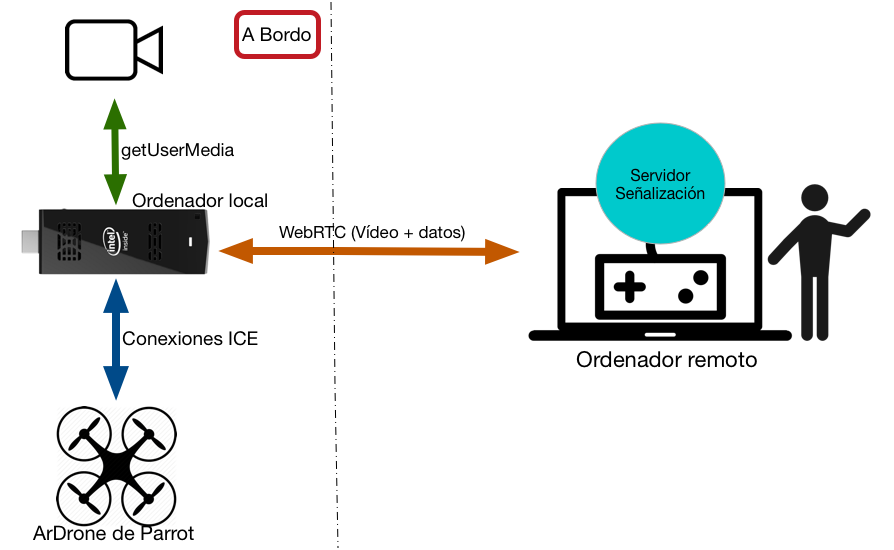
\includegraphics[width=0.7\textwidth]{esquema_experimento_abordo}
\caption{Esquema de la configuración del experimento.}
\label{fig:esquemaexperimentoabordo}
\end{figure}


En la figura \ref{fig:elementosabordo} se muestra la configuración de todos los elementos que hemos colocado a bordo del drone. Como se puede observar también hemos incluido un hub USB ya que es necesario al disponer el \emph{computer stick} de un único puerto USB y necesitar al menos dos, uno para la cámara y otro para el ratón en el momento que configuramos el navegador. Puede ver el montaje final en este vídeo\footnote{\url{http://jderobot.org/Irodmar-tfg#Experiment_Setup}} de la mediawiki.\\

\begin{figure}[h!]
\centering
\includegraphics[width=0.8\textwidth]{elementos_abordo}
\caption{Configuración de los elementos a bordo del drone.}
\label{fig:elementosabordo}
\end{figure}


Este experimento ha sido fallido, únicamente por las capacidades de vuelo que nos ofrece el drone. Entre los dispositivos que hemos colocado a bordo superamos la carga máxima de pago que permite este cuadricóptero. En lo que al funcionamiento de la aplicación se refiere ha funcionado perfectamente ya que en el par remoto obteníamos las imágenes y datos de vuelo procedentes del drone, y al ejecutar la orden de despegue el cuadricóptero ha intentado levantar el vuelo sin conseguirlo.\\

\begin{figure}[h!]
\centering
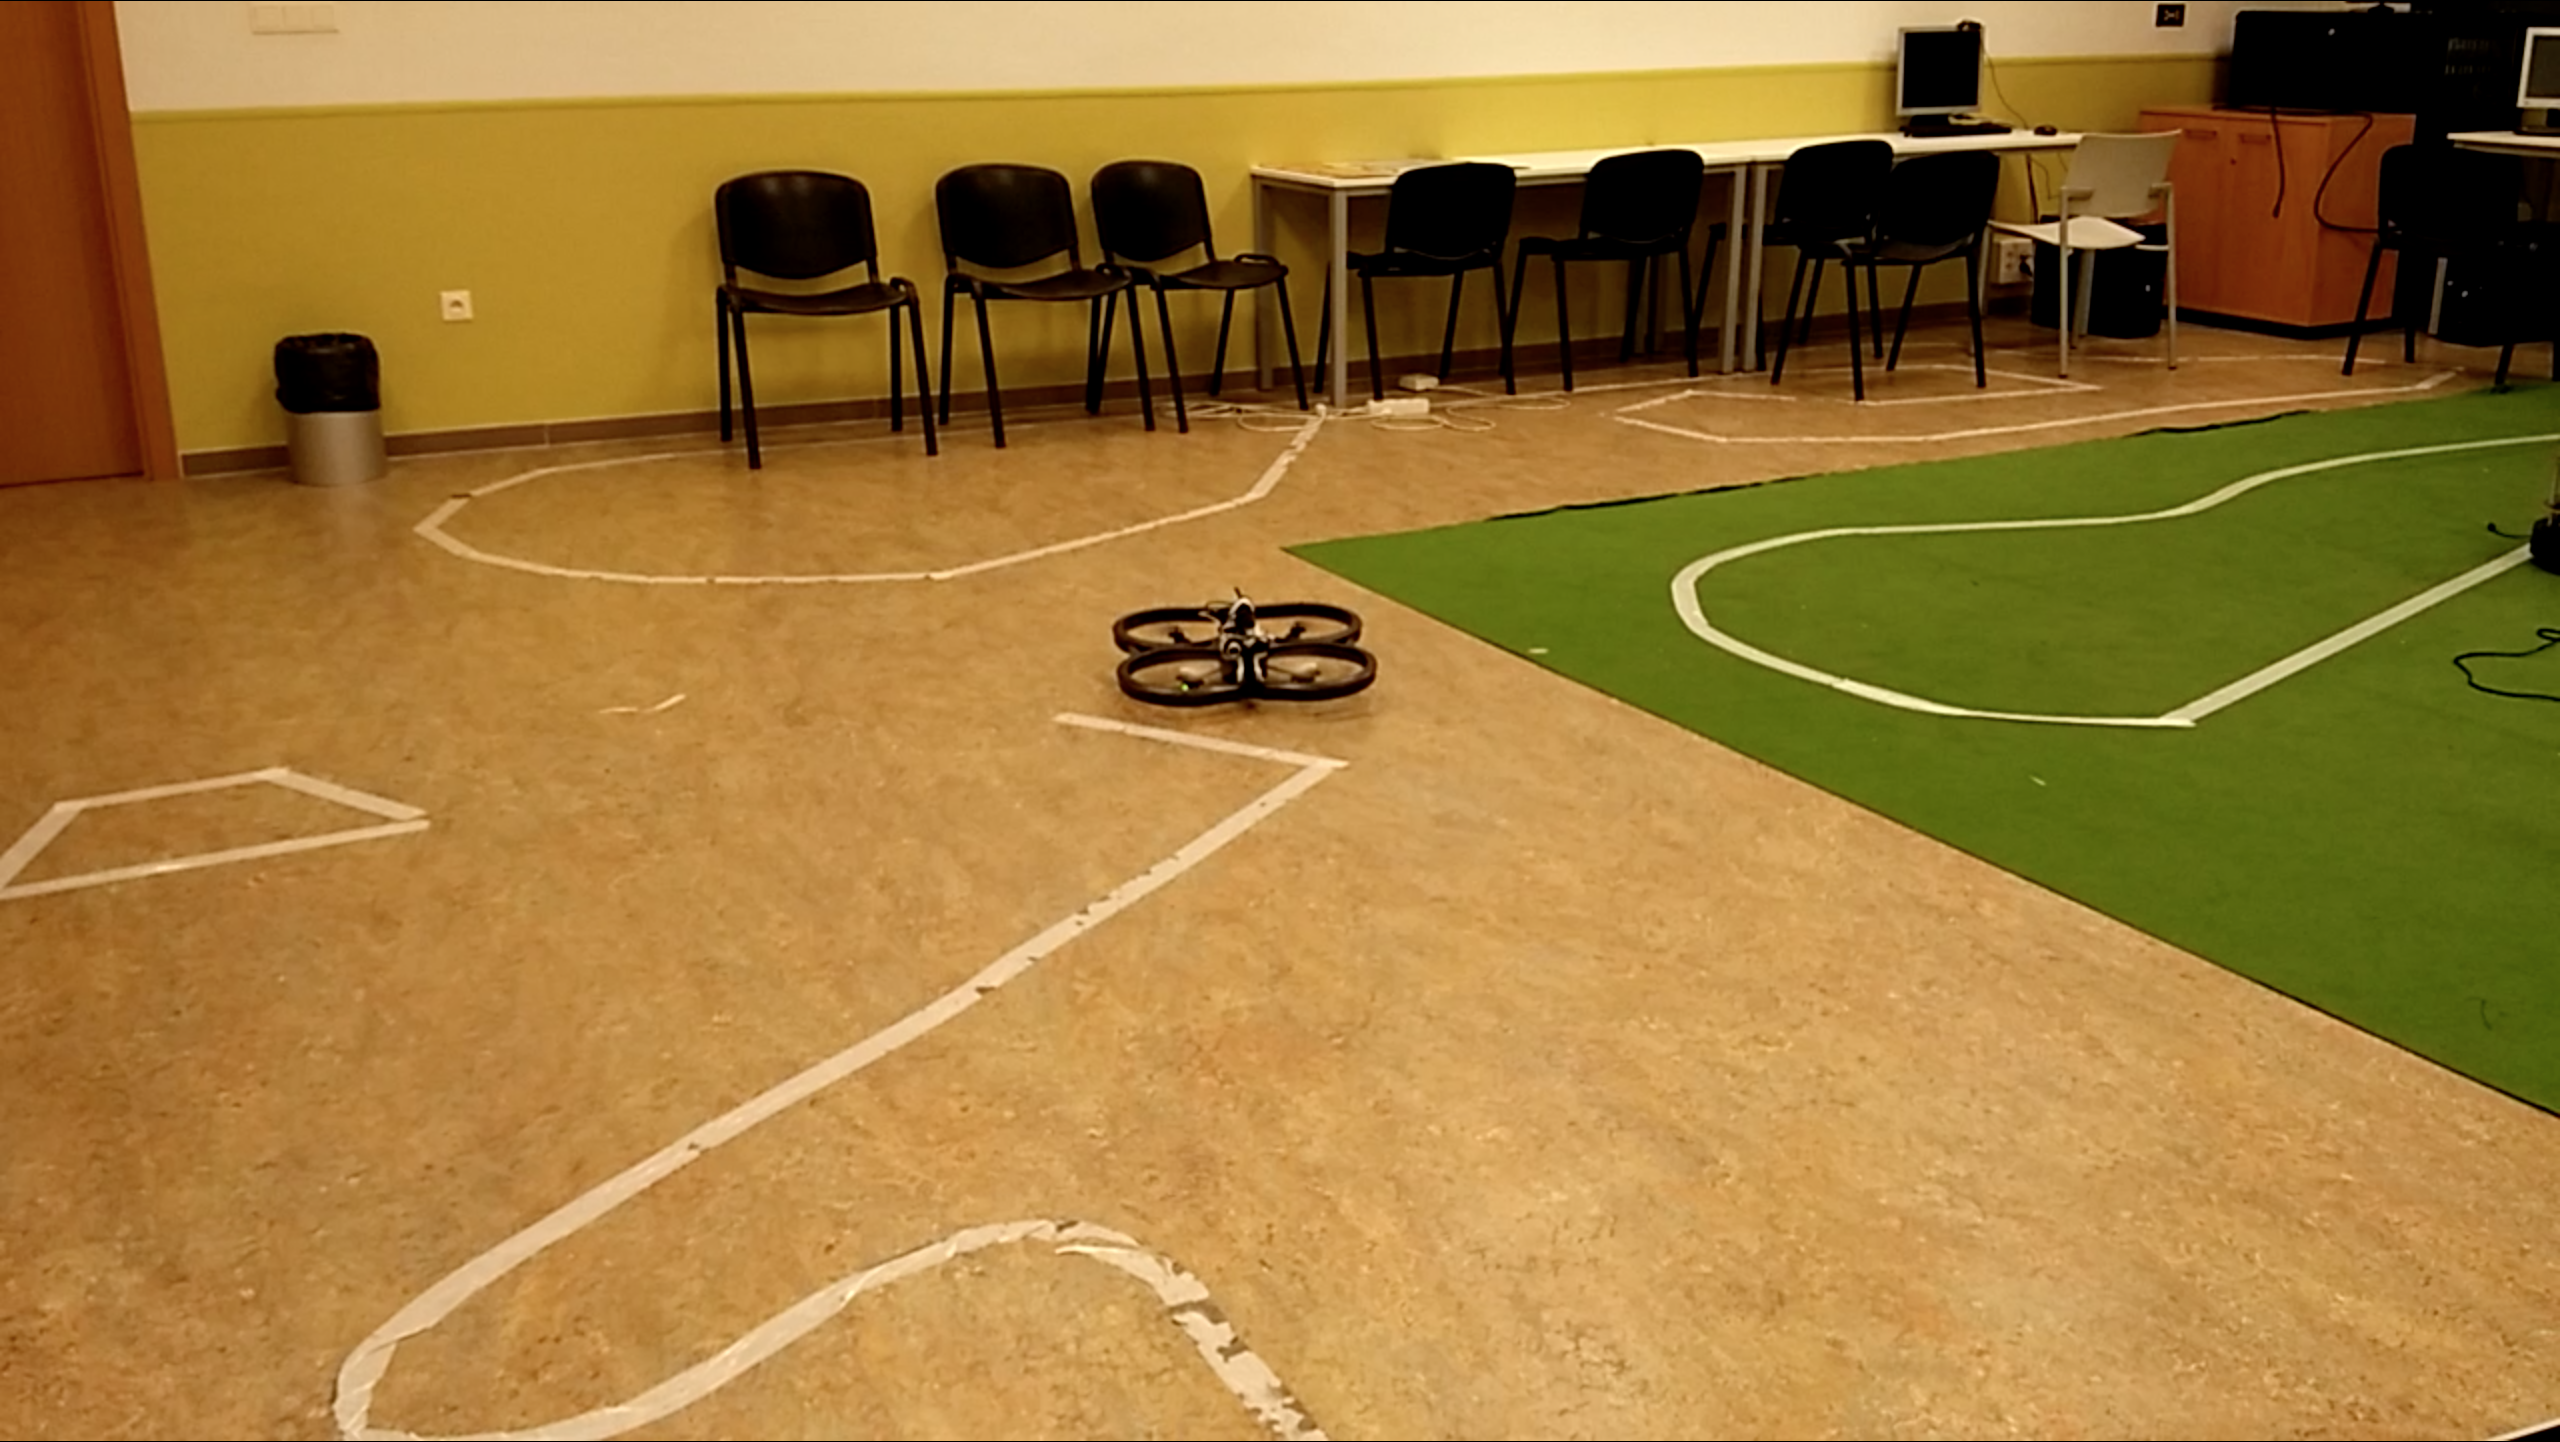
\includegraphics[width=0.7\textwidth]{experimento_abordo}
\caption{ArDrone no levanta el vuelo por exceso de peso.}
\label{fig:experimentoabordo}
\end{figure}

La figura \ref{fig:experimentoabordo} es un fotográma del vídeo\footnote{\url{http://jderobot.org/Irodmar-tfg#Attemp_of_flying}} que se grabó durante el experimento. En ella se ve al drone intentando levantar el vuelo. Para comprobar que el desarrollo funciona se optó por realizar otra prueba de vuelo en la que se cogía con las manos el drone y se le movía para observar que tanto la cámara a bordo cómo los relojes de vuelo variaban en el navegador remoto. La figura \ref{fig:pruebaexperimentoabordo} muestra un fotograma del vídeo\footnote{\url{http://jderobot.org/Irodmar-tfg#Testing_the_development}} en el que se realizan estas comprobaciones.\\

\begin{figure}[h!]
\centering
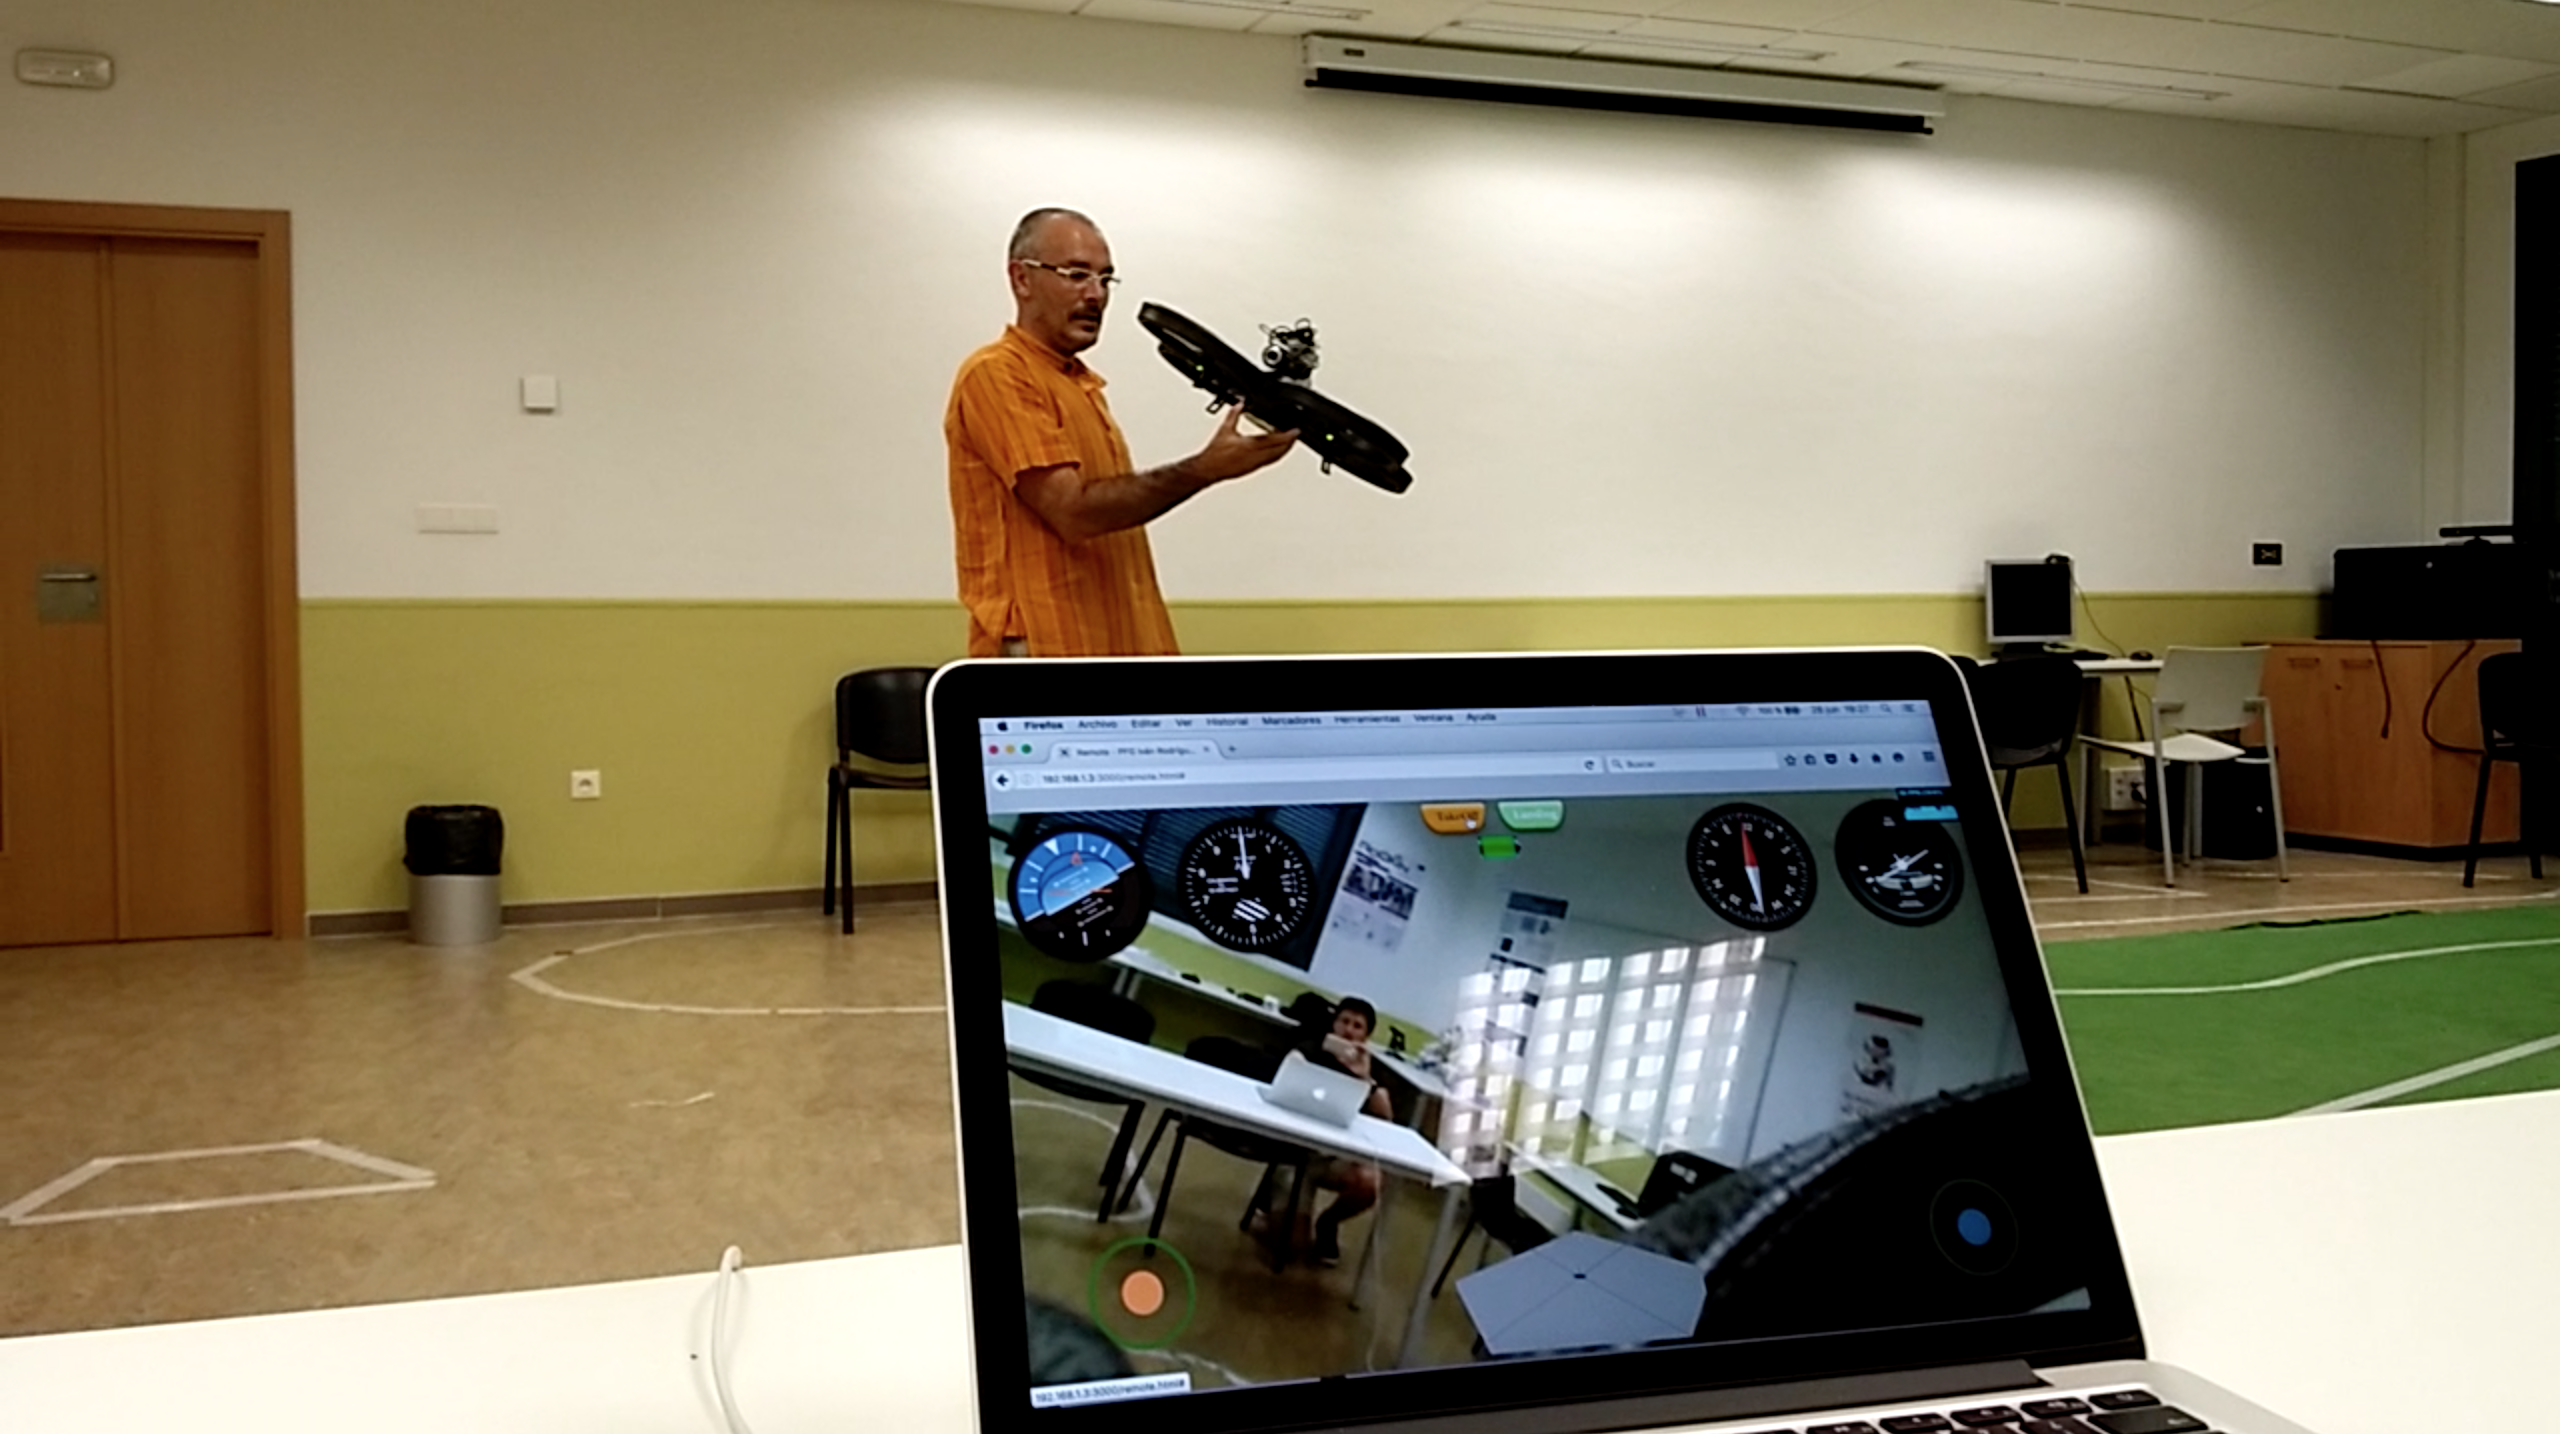
\includegraphics[width=0.7\textwidth]{pruebas_experimento_abordo}
\caption{Comprobación del funcionamiento de la aplicación.}
\label{fig:pruebaexperimentoabordo}
\end{figure}

\section{Vuelos con multidispositivos}

Como tercer y último experimento hemos probado a volar el drone utilizando dispositivos móviles. WebRTC tiene soporte para dispositivos móviles y los elementos de control los hemos desarrollado también para dispositivos táctiles, podemos utilizarlos como par remoto, par local o ambos. Al igual que el experimento anterior se ha realizado en dos pasos. Primero sin colocar el dispositivo a bordo del drone para confirmar su correcto funcionamiento y posteriormente repitiéndolo con el dispositivo a bordo. Realizar experimentos con dispositivos móviles implica la necesidad de la utilización de un ordenador de apoyo que será el que ejecute tanto el servidor de señalización para WebRTC cómo \texttt{ardrone\_server}.\\


\begin{figure}[h!]
\centering
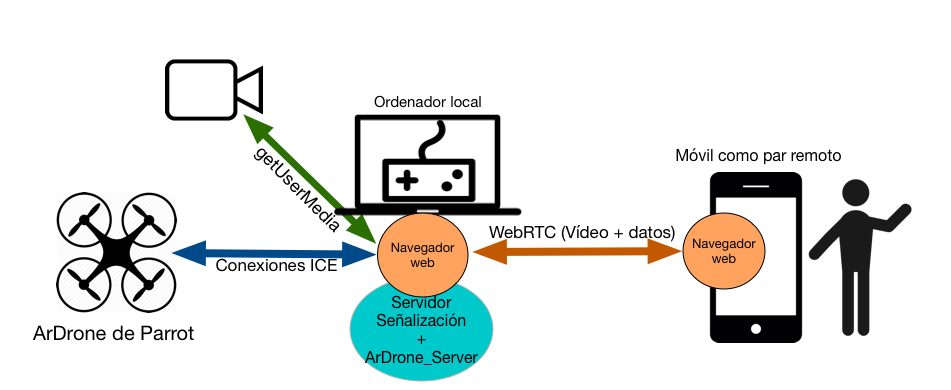
\includegraphics[width=0.8\textwidth]{esquema_experimento_multidispositivo_1}
\caption{Esquema del experimento con móvil como par remoto.}
\label{fig:esquemaexperimentomultidispositivo}
\end{figure}


Como primer experimento se ha utilizado un ordenador portátil como par local, encargado por un lado de estableciendo la conexion con el drone y de acceder a la cámara, en este caso la incorporada en el portátil, y por otro lado de correr los servidores de señalización y \texttt{ardrone\_server}. Como par remoto para teleoperar el drone se ha utilizado un teléfono móvil. En la figura \ref{fig:esquemaexperimentomultidispositivo} se detalla el esquema de este experimento.\\


En la figura \ref{fig:experimentodronemultidispositivo1} se puede apreciar un instante del experimento cuyo vídeo se encuentra en la mediawiki\footnote{\url{http://jderobot.org/Irodmar-tfg\#Flying\_with\_a\_mobile\_like\_Remote\_PC}}. En la figura \ref{fig:secexp3} podemos ver la secuencia de movimiento del drone teleoperado con un dispositivo móvil.\\

\begin{figure}[h!]
\centering
\includegraphics[width=0.9\textwidth]{experimentodronemultidispositivo1}
\caption{Experimento con móvil como par remoto.}
\label{fig:experimentodronemultidispositivo1}
\end{figure}


\begin{figure}[h!]
\centering
  \begin{subfigure}[]{48mm}
    \includegraphics[width=48mm]{sec_exp3_1}
  \end{subfigure}
  \hspace{1pt}
  \begin{subfigure}[]{48mm}
    \includegraphics[width=48mm]{sec_exp3_2}
  \end{subfigure}
    \hspace{1pt}
    \begin{subfigure}[]{48mm}
    \includegraphics[width=48mm]{sec_exp3_3}
  \end{subfigure}
    \caption{Secuencia de movimiento del experimento con dispositivo móvil como par remoto.}
  \label{fig:secexp3}
\end{figure}


\newpage
El segundo experimento (figura \ref{fig:esquemaexperimentomultidispositivo2}) es a la inversa, se utiliza un ordenador portátil como par remoto y un teléfono móvil como par local.

\begin{figure}[h!]
\centering
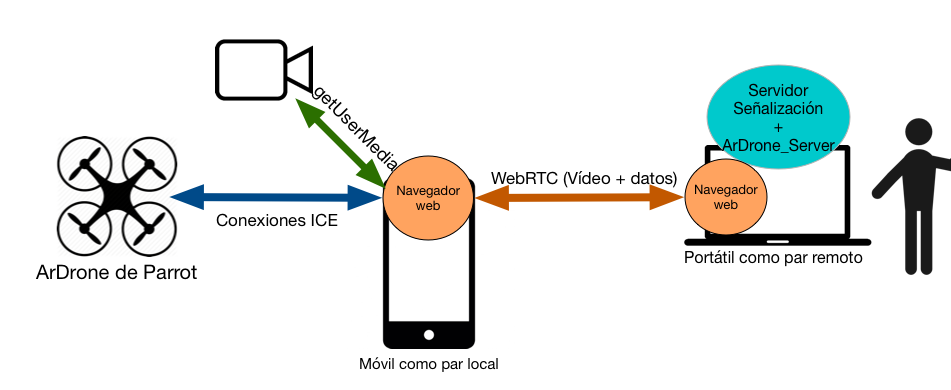
\includegraphics[width=0.8\textwidth]{experimento_multidispositivo2}
\caption{Esquema del experimento con móvil como par local.}
\label{fig:esquemaexperimentomultidispositivo2}
\end{figure}

En este configuración el ordenador portátil se utiliza también para ejecutar los servidores de señalización y \texttt{ardrone\_server}. El móvil se usa como par local, encargándose de establecer la conexion con el drone. En este caso las imágenes que se envían son de una de las dos cámaras del móvil, la delantera o la trasera, pudiendo elegir cualquiera de las dos. En este experimento el móvil lo colocamos sobre la mesa mirando hacia la posición en la que se encuentra en drone, por lo que en la pantalla del ordenador remoto le veremos moviéndose. La figura \ref{fig:experimentodronemultidispositivo2} muestra un momento del experimento que esta recogido en un vídeo en la mediawiki\footnote{\url{http://jderobot.org/Irodmar-tfg#Flying_with_a_mobile_like_Droner_PC}}. En la figura \ref{fig:secexp4} se muestra una secuencia del vuelo realizado.\\

\begin{figure}[h!]
\centering
\includegraphics[width=0.9\textwidth]{experimentodronemultidispositivo2}
\caption{Experimento con móvil como par local.}
\label{fig:experimentodronemultidispositivo2}
\end{figure}


\begin{figure}[h!]
\centering
  \begin{subfigure}[]{48mm}
    \includegraphics[width=48mm]{sec_exp4_1}
  \end{subfigure}
  \hspace{1pt}
  \begin{subfigure}[]{48mm}
    \includegraphics[width=48mm]{sec_exp4_2}
  \end{subfigure}
    \hspace{1pt}
    \begin{subfigure}[]{48mm}
    \includegraphics[width=48mm]{sec_exp4_3}
  \end{subfigure}
    \caption{Secuencia de movimiento del experimento con dispositivo móvil como par local.}
  \label{fig:secexp4}
\end{figure}

Se ha desestimado la realización del experimento en el que situamos el móvil a bordo del drone debido a la dificultad de colocarlo en posición vertical para que la cámara apunte desde la parte delantera del drone. La única posición dónde podría colocarse es en un extremo del cuadricóptero lo que causaría una descompensación de cargas dando lugar a que el drone no pudiese estabilizar el vuelo.\\

